\chapter{Concept Geometry via Contrastive Residual-Stream Analysis}
\label{sec:concept_geometry}

The reproducibility experiments in the previous chapter are guided by prior
knowledge of how circuits are expected to behave. However, interpreting a 
model's internal representations without such prior knowledge is challenging, 
as it might require statistics over many prompts, layers, and token positions,
 as well as creating hypotheses about the computation.
This chapter addresses a
more general problem, namely where in the network 
a concept first appears, at which token positions it is encoded,
 which transcoder features carry it, and how it evolves.

We use matched prompt pairs differing in one property to extract contrastive
residual-stream directions at each layer and anchor position.  We examine
inter-layer delta similarities to assess whether the direction is stable
across depth or undergoes representational rotation, and compare against a
permutation null baseline to separate genuine concept signal from artefacts
of the contrastive procedure.  We then project the directions onto transcoder
features to identify which sparse features align with the concept, and apply
causal patching as a complementary test of whether the direction is sufficient
to redirect the output.  We analyse three arithmetic tasks --- carry
detection, GCD divisibility, and residue class membership --- to study how
this geometry changes with problem structure.

\section{Contrastive Dataset}
\label{sec:concept_pairs}

For each concept we build matched prompt pairs \((x_i^+,x_i^-)\). The positive
prompt contains the target property. The negative prompt removes that property
while preserving the syntax, length, scale, and answer format as closely as
possible. This prevents the mean residual-stream difference from being dominated
by incidental token changes.

The prompt template is retained only when Qwen3-4B reaches at least 10\%
first-token accuracy. This threshold verifies that the model minimally respects the
output format. Since the first answer token
expresses the result, interventions are evaluated by their effect on that token, or
on a few subsequent tokens that are expected to capture the computation.

\begin{table}[ht!]
\centering
\setlength{\tabcolsep}{4pt}
\footnotesize
\begin{tabular}{@{}l l l l r r r@{}}
\toprule
Concept & Template
        & Positive
        & Negative
        & $N$
        & Acc.
        & $\bar{p}$ \\
\midrule
Carry
  & {\sffamily\scriptsize what is \{a\}+\{b\}? Answer:}
  & $a_0{+}b_0\!\geq\!10$
  & $a_0{+}b_0\!<\!10$
  & 99 & 100\% & 0.92 \\[3pt]
GCD
  & {\sffamily\scriptsize the gcd of \{a\} and 7 is:}
  & $\gcd(a,7)=7$
  & $\gcd(a,7)=1$
  & 100 & 86\% & 0.50 \\[3pt]
Res.\ class
  & {\sffamily\scriptsize calc: \{a\}\%7=}
  & $a \equiv 1 \pmod{7}$
  & $a \not\equiv 1 \pmod{7}$
  & 100 & 12\% & 0.12 \\
\bottomrule
\end{tabular}
\caption{Contrastive prompt sets.  Each pair contributes one positive and one
negative prompt.  Accuracy and $\bar{p}$ are measured on the first
answer token.}
\label{tab:concept_pairs}
\end{table}

\section{Residual-Stream Concept Delta}
\label{sec:concept_delta}

Let \(h_{l,t}(x) \in \mathbb{R}^d\) be the residual-stream vector at layer \(l\)
and token position \(t\). Rather than fixing one token position for analysis, 
we scan candidate positions \(\mathcal{T}\),
as the model processes different aspects of the computation at each token.

For anchor \(t^*\), the layer-wise concept delta is
\begin{equation}
\delta_l
=
\frac{1}{N}\sum_{i=1}^{N} h_{l,t^*}(x_i^+)
-
\frac{1}{N}\sum_{i=1}^{N} h_{l,t^*}(x_i^-)
=
\mathbb{E}[h_{l,t^*}(x^+)]-\mathbb{E}[h_{l,t^*}(x^-)].
\label{eq:concept_delta}
\end{equation}
Equivalently, if \(\Delta h_{i,l}=h_{l,t^*}(x_i^+)-h_{l,t^*}(x_i^-)\), then
\(\delta_l=N^{-1}\sum_i \Delta h_{i,l}\). The trajectory \((\delta_l)_{l=0}^{L-1}\) shows how the contrast changes through
the network. Under the linear representation hypothesis \citep{park2023linear},
\(\delta_l\) approximates a concept axis when the positive and
 negative prompts differ in only one property and the
concept is linearly separable at that layer.

\section{Layer and Anchor Metrics}
\label{sec:delta_metrics}

The simplest measure of concept strength at layer $l$ is the delta norm
\begin{equation}
D_l = \lVert \delta_l \rVert_2.
\label{eq:delta_norm}
\end{equation}
Since raw residual norms tend to grow with depth, we divide by the mean
activation norm at the same layer,
\begin{equation}
\mu_l^{\mathrm{act}} = \mathbb{E}_{x}\!\left[\lVert h_{l,t^*}(x)\rVert_2\right],
\label{eq:mean_act_norm}
\end{equation}
and use
\begin{equation}
D_l^{\mathrm{act}} = \frac{D_l}{\mu_l^{\mathrm{act}} + \varepsilon}.
\label{eq:act_norm_delta}
\end{equation}
To compare anchors with different absolute scale, each trajectory is divided by
its own maximum,
\begin{equation}
\tilde{D}_l^{\mathrm{act}}
=
\frac{D_l^{\mathrm{act}}}{\max_j D_j^{\mathrm{act}} + \varepsilon}
\in [0,1].
\label{eq:double_norm}
\end{equation}

High \(\tilde{D}_l^{\mathrm{act}}\) mark layers where the concept delta is
large relative to the residual-stream scale. Different anchor positions
may show broader or more localised patterns, as in Figure~\ref{fig:norm_comparison}. 

\begin{figure}[ht!]
  \centering
  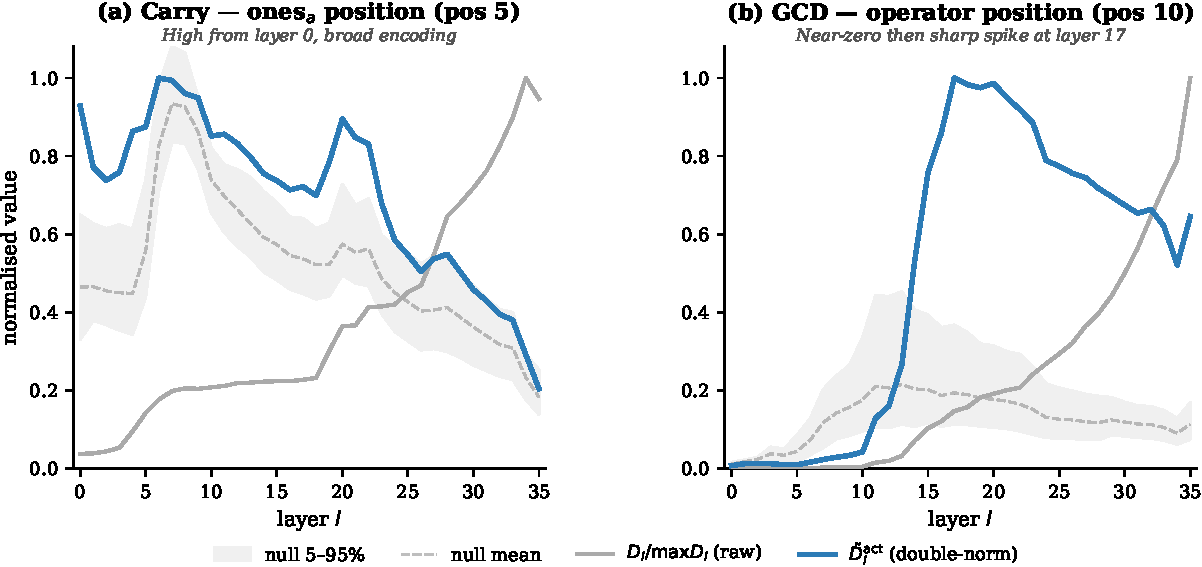
\includegraphics[width=\textwidth]{Pages/Figures/norm_comparison.pdf}
  \caption{Delta norms scaled to $[0,1]$, before and after division by the
  mean activation norm.  Activation normalisation reveals that the carry
  direction is broad across layers while the GCD direction is localised.}
  \label{fig:norm_comparison}
\end{figure}

% We also measure how concentrated the delta norm is across layers. Given
% \(l^*=\arg\max_l D_l\), the \textit{sharpness} score is
% \begin{equation}
% \operatorname{sharp}(t^*)
% =
% \frac{\sum_{l=\max(0,l^*-1)}^{\min(L-1,l^*+1)} D_l}
%      {\sum_{l=0}^{L-1} D_l + \varepsilon}.
% \label{eq:sharpness}
% \end{equation}
% High sharpness indicates a narrow processing window, and low sharpness can indicate a
% diffuse direction, weak separation, or a stable representation present across many
% layers, depending on expected value of \(\tilde{D}_l^{\mathrm{act}}\).

The \textbf{inter-layer cosine similarity} matrix shows whether the direction itself is stable,
\begin{equation}
C_{l,m}
=
\frac{\delta_l \cdot \delta_m}
       {\lVert\delta_l\rVert_2\,\lVert\delta_m\rVert_2 + \varepsilon}.
\label{eq:layer_cosine}
\end{equation}
A high-similarity block indicates one stable concept axis, while a two-block structure indicates
a rotation at the boundary between blocks, and a diffuse diagonal indicates gradual
rotation.

\citet{panickssery2024steeringllama2contrastive} report a diffuse diagonal pattern
for steering vectors in Llama 2, which is similar to the residue-class heatmap 
in Figure~\ref{fig:cosim_patterns}(c). However, we show that different tasks and anchors, such as
carry and GCD heatmaps in Figure~\ref{fig:cosim_patterns}(a) and (b) respectively, 
exhibit more structured patterns, with high-similarity blocks or sharper representational rotations.

\begin{figure}[ht!]
  \centering
  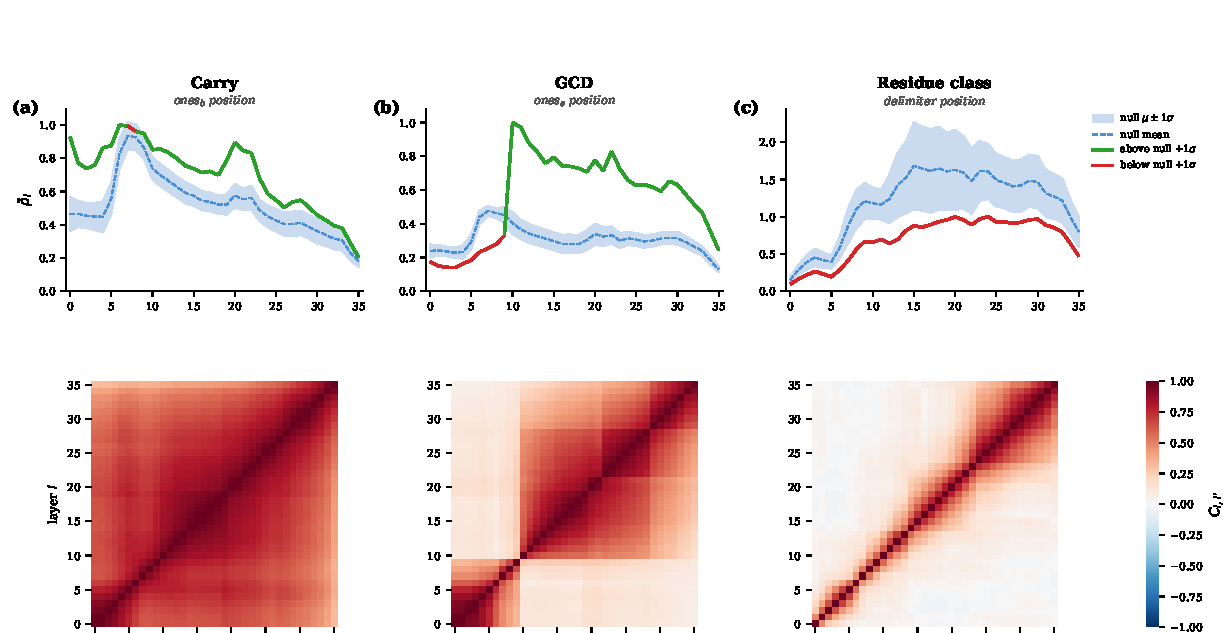
\includegraphics[width=\textwidth]{Pages/Figures/cosim_patterns_abc.pdf}
  \caption{Normalised delta trajectories and inter-layer cosine matrices.  Carry
  shows a stable direction, GCD shows a block transition, and residue class remains
  below the null band with only a diffuse diagonal.}
  \label{fig:cosim_patterns}
\end{figure}

% To select anchors, we compute the non-monotonicity score
% \begin{equation}
% \mathrm{nm}(t^*)
% =
% \max_{l}
% \min\!\left(
%   c_l - \min_{j < l} c_j,\quad
%   c_l - \min_{j > l} c_j
% \right),
% \label{eq:nonmonotonicity}
% \end{equation}
% where \(c_l = \tilde{D}_l^{\mathrm{act}}\).

\subsection{Null Permutation Test}
\label{sec:null_permutation}

A contrastive scan can create apparent directions even when labels are unrelated
to the concept. We estimate this background by permuting positive and negative
labels and recomputing the trajectory. For permutation \(\pi\), let
\(\delta_l^\pi\) be the resulting delta. The null distribution for statistic
\(q_l\) is
\begin{equation}
\left\{q_l(\delta^{\pi}) : \pi=1,\ldots,P\right\}.
\label{eq:null_distribution}
\end{equation}

Observed scores are compared against the null distribution.  A layer delta norm
above the null range suggests concept-specific signal beyond what generic
prompt variation produces.  A layer within or below the null range indicates
 that the binary contrast used
does not produce a discriminative direction at that anchor.
% However, the model may still perform
%  computation relevant to the task at that position.

\subsection{Causal Tests}
\label{sec:causal_validation}

\paragraph{Positive-to-Negative Activation Patching.}

To provide a causal sufficiency test, for each pair \((x_i^+,x_i^-)\) and
layer \(l\), we insert the positive residual vector at the anchor into the
negative forward pass,
\[
h_{l,t^*}(x_i^-) \leftarrow h_{l,t^*}(x_i^+).
\]
Let \(m(x)=\ell_{\mathrm{pos}}(x)-\ell_{\mathrm{neg}}(x)\) be the answer logit
margin at the final prediction position. The activation patching score is
\begin{equation}
S_l^{\mathrm{patch}}
=
\frac{1}{N}\sum_{i=1}^{N}
\left[m\!\left(\tilde{x}_{i,[l]}^-\right)-m(x_i^-)\right],
\label{eq:patch_score}
\end{equation}
where \(\tilde{x}_{i,[l]}^-\) is the negative prompt with the layer-\(l\) anchor
activation from the positive prompt. A positive score means that the
patched state moves the output toward the positive answer.

% \textcolor{red}{TODO: remove grad-dot-delta from report figs}
\paragraph{Gradient-dot-delta.}

As a first-order approximation to patching, we score each layer by the
inner product of the output-margin gradient and the mean concept delta,
\begin{equation}
S_l^{\mathrm{grad}}
=
\frac{1}{N}\sum_{i=1}^{N}
\nabla_{h_{l,t^*}}m(x_i^- )\cdot\delta_l.
\label{eq:grad_delta_score}
\end{equation}
This follows from the Taylor expansion
\begin{equation}
m(\tilde{x}_{i,[l]}^-)
\approx
m(x_i^-)
+
\nabla_{h_{l,t^*}}m(x_i^-)
\cdot
\left(h_{l,t^*}(x_i^+) - h_{l,t^*}(x_i^-)\right).
\label{eq:patch_taylor}
\end{equation}
When the two scores are similar, the output is locally linear along the concept
direction.  When they diverge, higher-order effects dominate or the mean
delta is a weak approximation of the individual pair differences.

\begin{figure}[ht!]
  \centering
  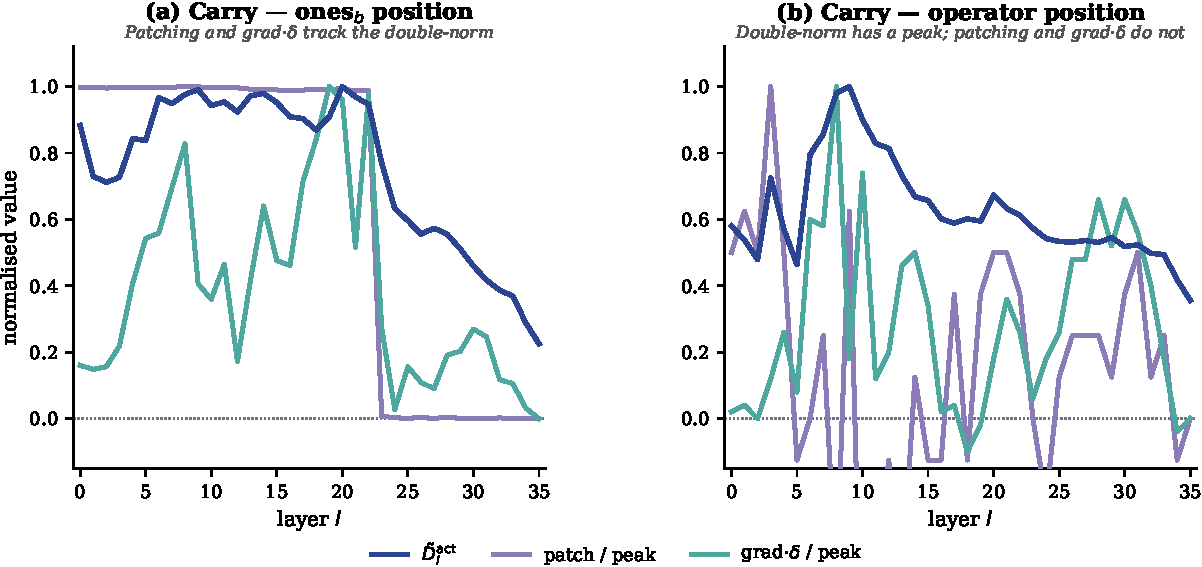
\includegraphics[width=\textwidth]{Pages/Figures/causal_overlay_comparison.pdf}
  \caption{Residual direction and activation patching for two anchors in the addition prompt.  
  The ones$_b$ anchor shows alignment of geometric and causal evidence.  The
  operator anchor shows no causal effect on the answer, reflecting low separability
  of the concept at that anchor.}
  \label{fig:causal_overlay_comparison}
\end{figure}

\subsection{Anchor Selection}
\label{sec:peak_selection}

We select anchor positions in two stages, to avoid computing
concept statistics for all token positions, given that 
many of which carry no concept signal. In the first stage, we rank all candidate
positions by mean inter-layer cosine similarity of \(\delta_l\) given by 
Equation \ref{eq:layer_cosine} and retain
the first six anchors. In the second stage, we score each by the combined criterion
\begin{equation}
S
=
\tilde{D}^{\mathrm{act}}
+
\max(0,\,D^{\mathrm{act}}-\mathrm{null})
+
S^{\mathrm{patch}},
\label{eq:anchor_score}
\end{equation}

as a final ranking of the six anchors, which we then
use to analyise the concept geometry.

\section{Transcoder Feature Projection}
\label{sec:feature_projection}

For each transcoder feature we project \(\delta_l\) onto its decoder and encoder
directions. The decoder projection quantifies whether the feature writes along the
concept direction and the encoder projection measures its sensitivity to the concept in
the incoming residual stream.

\paragraph{Decoder output alignment.}
The transcoder decomposes the post-block residual as
\begin{equation}
h_l^{\mathrm{post}}(x)
= h_l^{\mathrm{mid}}(x) + \sum_f z_{l,f}(x)\,w_{l,f}^{\mathrm{dec}},
\label{eq:transcoder_decomp}
\end{equation}
where \(h_l^{\mathrm{mid}}\) is the residual entering the MLP block.
Taking the contrastive mean difference,
\begin{equation}
\delta_l^{\mathrm{post}}
= \delta_l^{\mathrm{mid}} + \sum_f \Delta z_{l,f}\,w_{l,f}^{\mathrm{dec}},
\label{eq:delta_decomp}
\end{equation}
with \(\Delta z_{l,f}=\mathbb{E}[z_{l,f}(x^+)]-\mathbb{E}[z_{l,f}(x^-)]\).
Projecting onto a decoder vector \(w_{l,f'}^{\mathrm{dec}}\) gives
\begin{equation}
\delta_l^{\mathrm{post}}\cdot w_{l,f'}^{\mathrm{dec}}
=
\delta_l^{\mathrm{mid}}\cdot w_{l,f'}^{\mathrm{dec}}
+
\sum_f \Delta z_{l,f}
\underbrace{\bigl(w_{l,f}^{\mathrm{dec}}\cdot w_{l,f'}^{\mathrm{dec}}\bigr)}_{\text{decoder Gram matrix}},
\label{eq:dec_gram}
\end{equation}
or in matrix form \(\delta_l^{\mathrm{post}} W^{\mathrm{dec}\top} = \delta_l^{\mathrm{mid}} W^{\mathrm{dec}\top} + \Delta z_l\,(W^{\mathrm{dec}}W^{\mathrm{dec}\top})\).
 We rank features by the normalised cosine between the decoder direction and \(\delta_l^{\mathrm{post}}\),
\begin{equation}
\operatorname{cos}_{l,f}^{\mathrm{dec}}
=
\frac{w_{l,f}^{\mathrm{dec}} \cdot \delta_l^{\mathrm{post}}}
     {\lVert w_{l,f}^{\mathrm{dec}}\rVert_2\,\lVert\delta_l^{\mathrm{post}}\rVert_2 + \varepsilon}.
\label{eq:decoder_cosine}
\end{equation}

\paragraph{Encoder input alignment.}
Since \(\delta_l\) is measured on the output residual \(h_l^{\mathrm{post}}\) rather
than the MLP input \(h_l^{\mathrm{mid}}\), we treat encoder alignment as a secondary
statistic. The normalised cosine between the encoder direction and \(\delta_l\) is
\begin{equation}
\operatorname{cos}_{l,f}^{\mathrm{enc}}
=
\frac{w_{l,f}^{\mathrm{enc}} \cdot \delta_l}
     {\lVert w_{l,f}^{\mathrm{enc}}\rVert_2\,\lVert\delta_l\rVert_2 + \varepsilon},
\label{eq:encoder_cosine}
\end{equation}
which measures the sensitivity of feature \(f\) to the concept direction in the MLP input.

\paragraph{Combined feature score.}
We rank features by the sum of decoder and encoder alignment,
\begin{equation}
\sigma_{l,f}
=
\operatorname{cos}_{l,f}^{\mathrm{dec}}
+
\operatorname{cos}_{l,f}^{\mathrm{enc}}.
\label{eq:combined_cos}
\end{equation}
Features with \(\sigma_{l,f}>0\) are aligned with the positive class, while those with
\(\sigma_{l,f}<0\) are aligned with the negative class. Figures~\ref{fig:concept_summary_carry}--\ref{fig:concept_summary_residue} show
feature projections and decoder-aligned activations for a set of four chosen anchors of each
concept.

\begin{figure}[htbp]
\centering
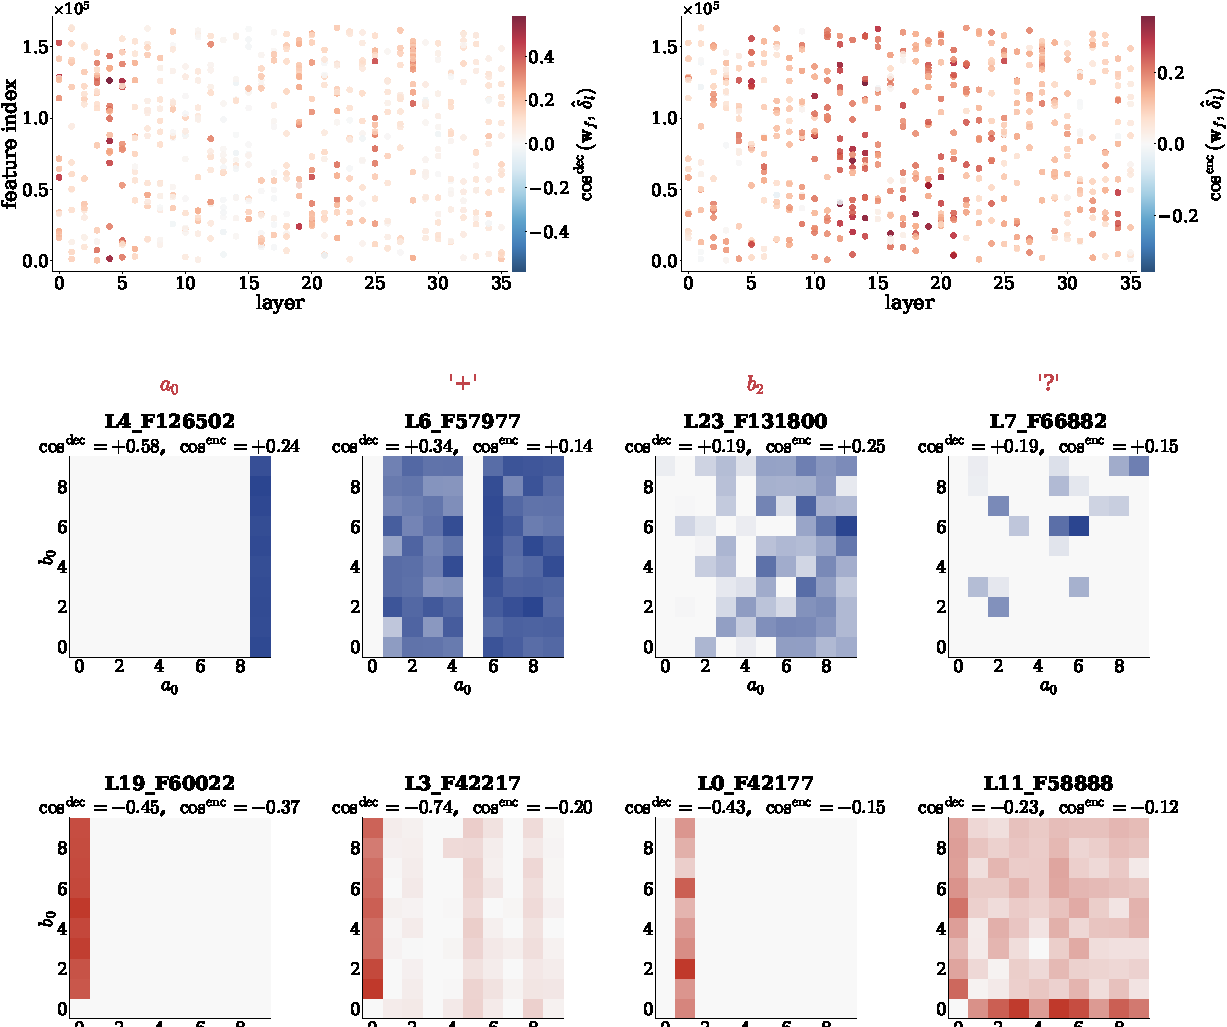
\includegraphics[width=\textwidth]{Pages/Figures/carry/concept_summary_T0_thesis.pdf}
\caption{Carry feature projections.  Decoder and encoder cosine identify features
aligned with the carry direction.  The activation grids show units-digit
detectors and carry-region detectors.}
\label{fig:concept_summary_carry}
\end{figure}

\begin{figure}[htbp]
\centering

\includegraphics[width=\textwidth]{Pages/Figures/gcd/concept_summary_T0_thesis.pdf}
\caption{GCD feature projections.  Several decoder-aligned features activate
selectively at \(a\equiv 0\pmod 7\), including features that appear at more than
one anchor.}
\label{fig:concept_summary_gcd}
\end{figure}

\begin{figure}[htbp]
\centering

\includegraphics[width=\textwidth]{Pages/Figures/residue_class/concept_summary_T0_thesis.pdf}
\caption{Residue-class feature projections.  The strongest projected features
often detect divisibility by seven rather than the selected residue class, which
links this scan to the GCD representation.}
\label{fig:concept_summary_residue}
\end{figure}

\section{Feature-Direction Interventions}
\label{sec:interventions}

We test projected features by modifying the raw MLP output along their decoder
directions. We avoid full transcoder reconstruction as it degrades
first-token accuracy. 

\paragraph{Feature-Output Ablation.}

For feature \(f\) with decoder direction \(w_{l,f}^{\mathrm{dec}}\), we compute its
activation \(z_{l,f}(x)\) and subtract the selected part of its decoder contribution
from the MLP output,
\begin{equation}
y_l(x) \leftarrow y_l(x) - (1-\alpha)\, z_{l,f}(x)\, w_{l,f}^{\mathrm{dec}},
\label{eq:ablation}
\end{equation}
where \(\alpha=0\) gives full ablation and \(\alpha=1\) leaves the model unchanged.

\paragraph{Decoder-Direction Injection.}

Injection adds the decoder direction at a fixed token position whether or not the
feature activates naturally,
\begin{equation}
y_l(x) \leftarrow y_l(x) + \delta_f\, w_{l,f}^{\mathrm{dec}}.
\label{eq:injection}
\end{equation}
The magnitude \(\delta_f\) is the mean natural activation
\(\bar{a}_f^+=\mathbb{E}[z_{l,f}(x^+)]\) resulted from scanning a set of 
concept pairs. 

\section{Empirical Results}
\label{sec:concept_results}

\subsection{Addition}
\label{sec:carry_results}

\paragraph{Carry Detection in Three-Digit Addition.}
% \textcolor{red}{TODO: add figs}
Carry-related concept directions are present  at the ones$_a$ and ones$_b$ anchor.
The delta norm peaks at layers 4--5, with secondary peaks at layers 19 and 22; the
cosine heatmap shows a block transition near layers 4--5 followed by a stable carry
direction in later layers. 

\paragraph{Ablation.}
Joint ablation of first ten projected features with \(\alpha=0\) reduces accuracy from 100\% to 47.8\% on the
23 activating prompts. Individual ablations have no effect, indicating functional
redundancy. The prediction shifts in Table~\ref{tab:carry_intervention} range from
\(-8\) to \(-11\), close to the units digit of the second operand, suggesting these
features encode part of the digit-level value entering the running sum.

\paragraph{Injection.}
Adding the four decoder directions at fixed magnitude \(\delta=5.0\) to 198
carry-negative prompts reduces accuracy from 100\% to 22.2\%, changing 154
predictions by \(+7\) or \(+8\) (Table~\ref{tab:carry_intervention}), as though
a carry were present despite \(a_0+b_0<10\).

\begin{table}[ht!]
\centering
\caption{Representative carry intervention effects at the ones$_b$ anchor.
Changed digits are bold.}
\label{tab:carry_intervention}
\begin{minipage}[t]{0.47\textwidth}
  \centering
  \small
  Joint ablation on carry-positive prompts\\[4pt]
  \begin{tabular}{@{}l r r r@{}}
  \toprule
  Prompt & Baseline & Ablated & $\Delta$ \\
  \midrule
  $289{+}201$ & $490$ & $4\mathbf{8}\mathbf{2}$ & $-8$ \\
  $649{+}132$ & $781$ & $7\mathbf{7}\mathbf{0}$ & $-11$ \\
  $669{+}411$ & $1080$ & $10\mathbf{7}\mathbf{2}$ & $-8$ \\
  $111{+}729$ & $840$ & $8\mathbf{3}0$ & $-10$ \\
  \bottomrule
  \end{tabular}
\end{minipage}
\hfill
\begin{minipage}[t]{0.47\textwidth}
  \centering
  \small
  Decoder injection on carry-negative prompts\\[4pt]
  \begin{tabular}{@{}l r r r@{}}
  \toprule
  Prompt & Baseline & Injected & $\Delta$ \\
  \midrule
  $200{+}531$ & $731$ & $73\mathbf{9}$ & $+8$ \\
  $280{+}201$ & $481$ & $48\mathbf{9}$ & $+8$ \\
  $640{+}132$ & $772$ & $77\mathbf{9}$ & $+7$ \\
  $280{+}502$ & $782$ & $78\mathbf{9}$ & $+7$ \\
  \bottomrule
  \end{tabular}
\end{minipage}
\end{table}

\paragraph{Fourier Structure in Carry Feature Grids.}
\label{sec:fourier_patterns}

Beyond the aggregate cosine ranking of Equation~\ref{eq:combined_cos}, we examine
individual transcoder features for digit-level structure, independent of whether
they rank highly under \(\sigma_{l,f}\). For every active feature \(f\) at every
layer \(l\), and at the ones$_b$ anchor, we scan operands \(a,b\) and aggregate the
post-ReLU activation into a \(10\times10\) grid,
\begin{equation}
X_{l,f}[a_0,b_0]
=
\mathbb{E}\bigl[z_{l,f}(x) \mid a\bmod 10=a_0,\; b\bmod 10=b_0\bigr],
\label{eq:fourier_grid}
\end{equation}
min-max normalised to \([0,1]\) per feature.  Writing
\(\hat X_{l,f}[u,v]\) for the mean-subtracted 2D FFT of \(X_{l,f}\), each frequency
pair corresponds to a cosine mode \(\cos\bigl(2\pi(ua_0+vb_0)/10+\varphi_{u,v}\bigr)\),
and we group modes into six symmetry classes: \emph{row}- or \emph{column}-only
(\(v{=}0\) or \(u{=}0\), a function of a single digit), \emph{row-} or
\emph{column-parity} at the Nyquist frequency (\(|u|{=}5,v{=}0\) or \(u{=}0,|v|{=}5\),
i.e.\ \((-1)^{a_0}\) or \((-1)^{b_0}\)), global \emph{parity} (\(|u|{=}|v|{=}5\), i.e.\
\((-1)^{a_0+b_0}\)), \emph{iso-sum} (\(u{=}v\), a function of \(a_0{+}b_0\)),
\emph{iso-difference} (\(u{=}{-}v\), a function of \(b_0{-}a_0\)), or \emph{mixed}. The reconstruction from the top-\(K\) modes by amplitude is
\begin{equation}
\hat{X}_{l,f}^{(K)}[a_0,b_0]
=
\bar X_{l,f} + \sum_{k=1}^{K} A_k\cos\!\left(\frac{2\pi(u_ka_0+v_kb_0)}{10}+\varphi_k\right),
\label{eq:fourier_recon}
\end{equation}
and we define the structured-energy fraction of a feature as the share of its non-DC
spectral power carried by modes with an explicit digit-pair symmetry,
\begin{equation}
S_{l,f}
=
\frac{\displaystyle\sum_{(u,v)\,\in\,\{\text{parity, row-par., col-par., iso-sum, iso-diff.}\}} \bigl|\hat X_{l,f}[u,v]\bigr|^2}
     {\displaystyle\sum_{(u,v)\neq(0,0)} \bigl|\hat X_{l,f}[u,v]\bigr|^2}.
\label{eq:structured_energy}
\end{equation}
After scanning active features at every layer, we retain those with
\(S_{l,f}>0.6\). The selected set concentrates almost entirely in layers 12--14 and
21, at or beyond the layers where the delta trajectory in
Figure~\ref{fig:cosim_patterns}(a) reaches its maximum.

Figure~\ref{fig:fourier_selection} and Table~\ref{tab:fourier_features} show eight example features from this set, each
with its activation grid alongside the smallest reconstruction (up to \(K{=}6\)
modes in Equation~\ref{eq:fourier_recon}) reaching \(R^2\geq0.90\). 

\begin{table}[ht!]
\centering
\small
\begin{tabular}{@{}llll@{}}
\toprule
Feature & Layer & Symmetry category & Closed-form predicate \\
\midrule
$F_{1468}$   & 12 & row-parity      & $a_0 \bmod 2 = 1$ \\
$F_{30390}$  & 21 & column-parity   & $a_0 \bmod 2 = 1 \text{ and } b_0 \bmod 2 = 1$ \\
$F_{57984}$  & 13 & iso-difference  & $a_0 - b_0 = 0$ \\
$F_{114215}$ & 14 & iso-sum         & $a_0 + b_0 = 10$ \\
$F_{75746}$  & 13 & global parity   & $(a+b)\bmod 2 = 1$ \\
$F_{56616}$  & 13 & iso-difference  & $|a-b| \equiv 3 \pmod{10}$ \\
$F_{107956}$ & 13 & iso-difference  & $|a-b| \equiv 3 \pmod{10}$ \\
$F_{132660}$ & 13 & iso-sum         & $a+b \bmod 10 \in \{4,5,6\}$ \\
\bottomrule
\end{tabular}
\caption{Symmetry category of the eight features in Figure~\ref{fig:fourier_selection}
and the arithmetic predicate each appears to encode.}
\label{tab:fourier_features}
\end{table}
\clearpage
This structure invites comparison with the Fourier circuits reported in small models
trained from scratch on modular arithmetic. \citet{nanda2023progress} find that a
one-layer transformer trained purely on modular addition converges onto a small
shared set of low-frequency components, and \citet{zhong2023clock} show that the
resulting \emph{clock} algorithm reads the sum directly off the phase of one or two
dominant frequencies. In both accounts the structure is located in the
\emph{weights}, since the token embeddings organise into circles at a handful of
shared frequencies and every neuron's response follows from reading out those
directions. The structure found here instead lives in \emph{activation} space,
where individual transcoder features happen to respond to the operand grid as
approximately single Fourier modes, so the basis is an empirical property of the
dictionary's activation patterns rather than of the weights that produced them.

Joint ablation of most ranked 60 features by their structured energy does not change task accuracy (\(\Delta p = +0.003\)), indicating
causal dispensability within this subset. This suggests that while Qwen3-4B exhibits Fourier structure in the context
of addition tasks provided by our dataset,
 this structure is one capability among many, rather than a causal component.

\begin{figure}[ht!]
  \centering
  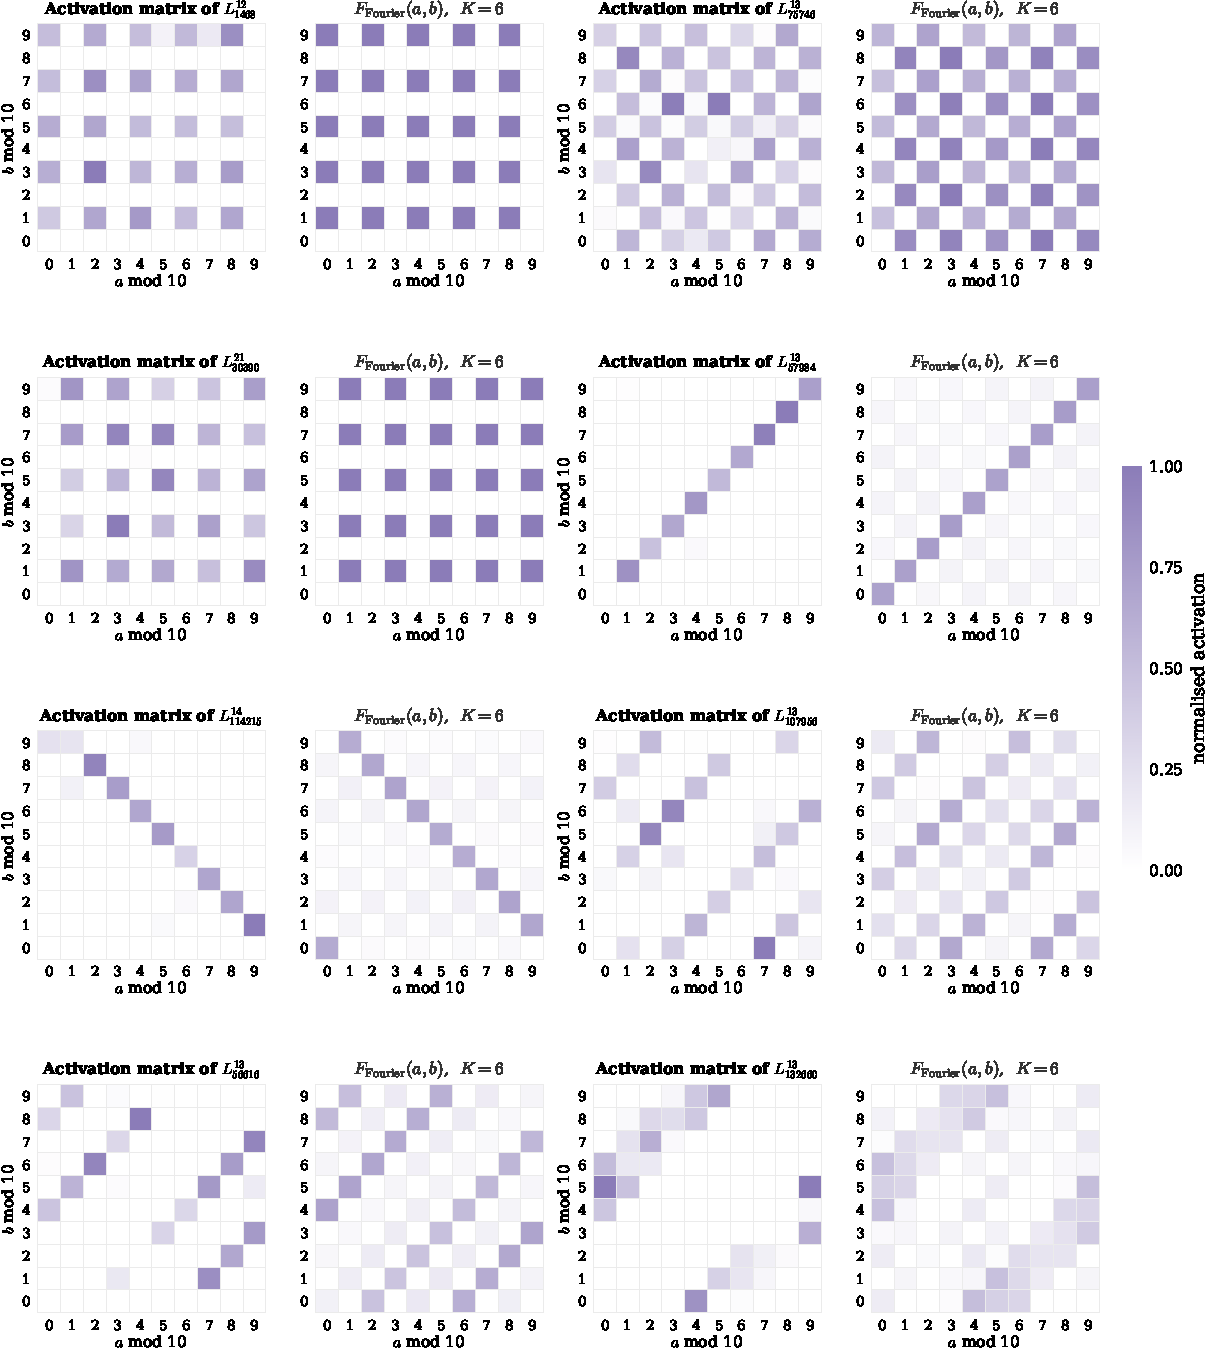
\includegraphics[width=\textwidth]{Pages/Figures/fourier_selection.pdf}
  \caption{Fourier-structured transcoder features at the carry ones$_b$ anchor,
  selected by structured-energy fraction \(S_{l,f}>0.6\)
  (Equation~\ref{eq:structured_energy}). Each feature is shown as an activation grid
  and its top-\(K\) Fourier approximation (Equation~\ref{eq:fourier_recon}), labelled
  by the number of modes \(K\) needed to reach \(R^2\geq0.90\).}
  \label{fig:fourier_selection}
\end{figure}

\subsection{GCD Divisibility by Seven}
\label{sec:gcd_results}

In Figure \ref{fig:concept_overview_gcd}(b), several anchors exceed the null permutation band, indicating the
binary component of this task. The inter-layer cosine matrix shows a block transition 
at layer 10 for the ones$_a$ anchor in Figure~\ref{fig:cosim_patterns}(b). This anchor
and layer position is also where projected features start exhibiting
 prime and co-prime patterns by seven. Since this position is reached before the operator (seven),
it is an indication that the model already has feature detectors for divisibility by seven for arbitrary integers, 
and that these features are
revealed by the nature of our contrastive prompts.

% Moreover, ablation of the first \textcolor{red}{X} features ranked by absolute cosine described in Equation
% \ref{eq:combined_cos} reduces accuracy from \textcolor{red}{X} to \textcolor{red}{X} 
% on the \textcolor{red}{X} activating prompts. This indicates that these feature are causally relevant 
% to the GCD by seven, even though they appear before the seven token.

\subsection{Residue-Class Membership Modulo Seven}
\label{sec:residue_results}

No anchor consistently exceeds the permutation null band for 
the residue-class contrast (\(a\equiv 1\pmod{7}\) 
versus \(a\not\equiv 1\pmod{7}\)). 
Figure~\ref{fig:concept_overview_residue}(c)
 shows that some of the strongest projected features detect divisibility
 by seven, similarly to the GCD divisibility results.
 
%  However, 
%  ablation of the first \textcolor{red}{X} strongest features \textcolor{red}{is}
%  causally not sufficient to change the output, 
%  as accuracy remains at \textcolor{red}{X} on the \textcolor{red}{X} activating prompts. This aspect
%  indicates that the lack of a binary component, as the residue-class membership
%  task is a multi-class problem, therefore the model does not learn a linear concept direction.

\clearpage
\begin{figure}[p]
\centering
\thispagestyle{empty}
\vspace*{\fill}
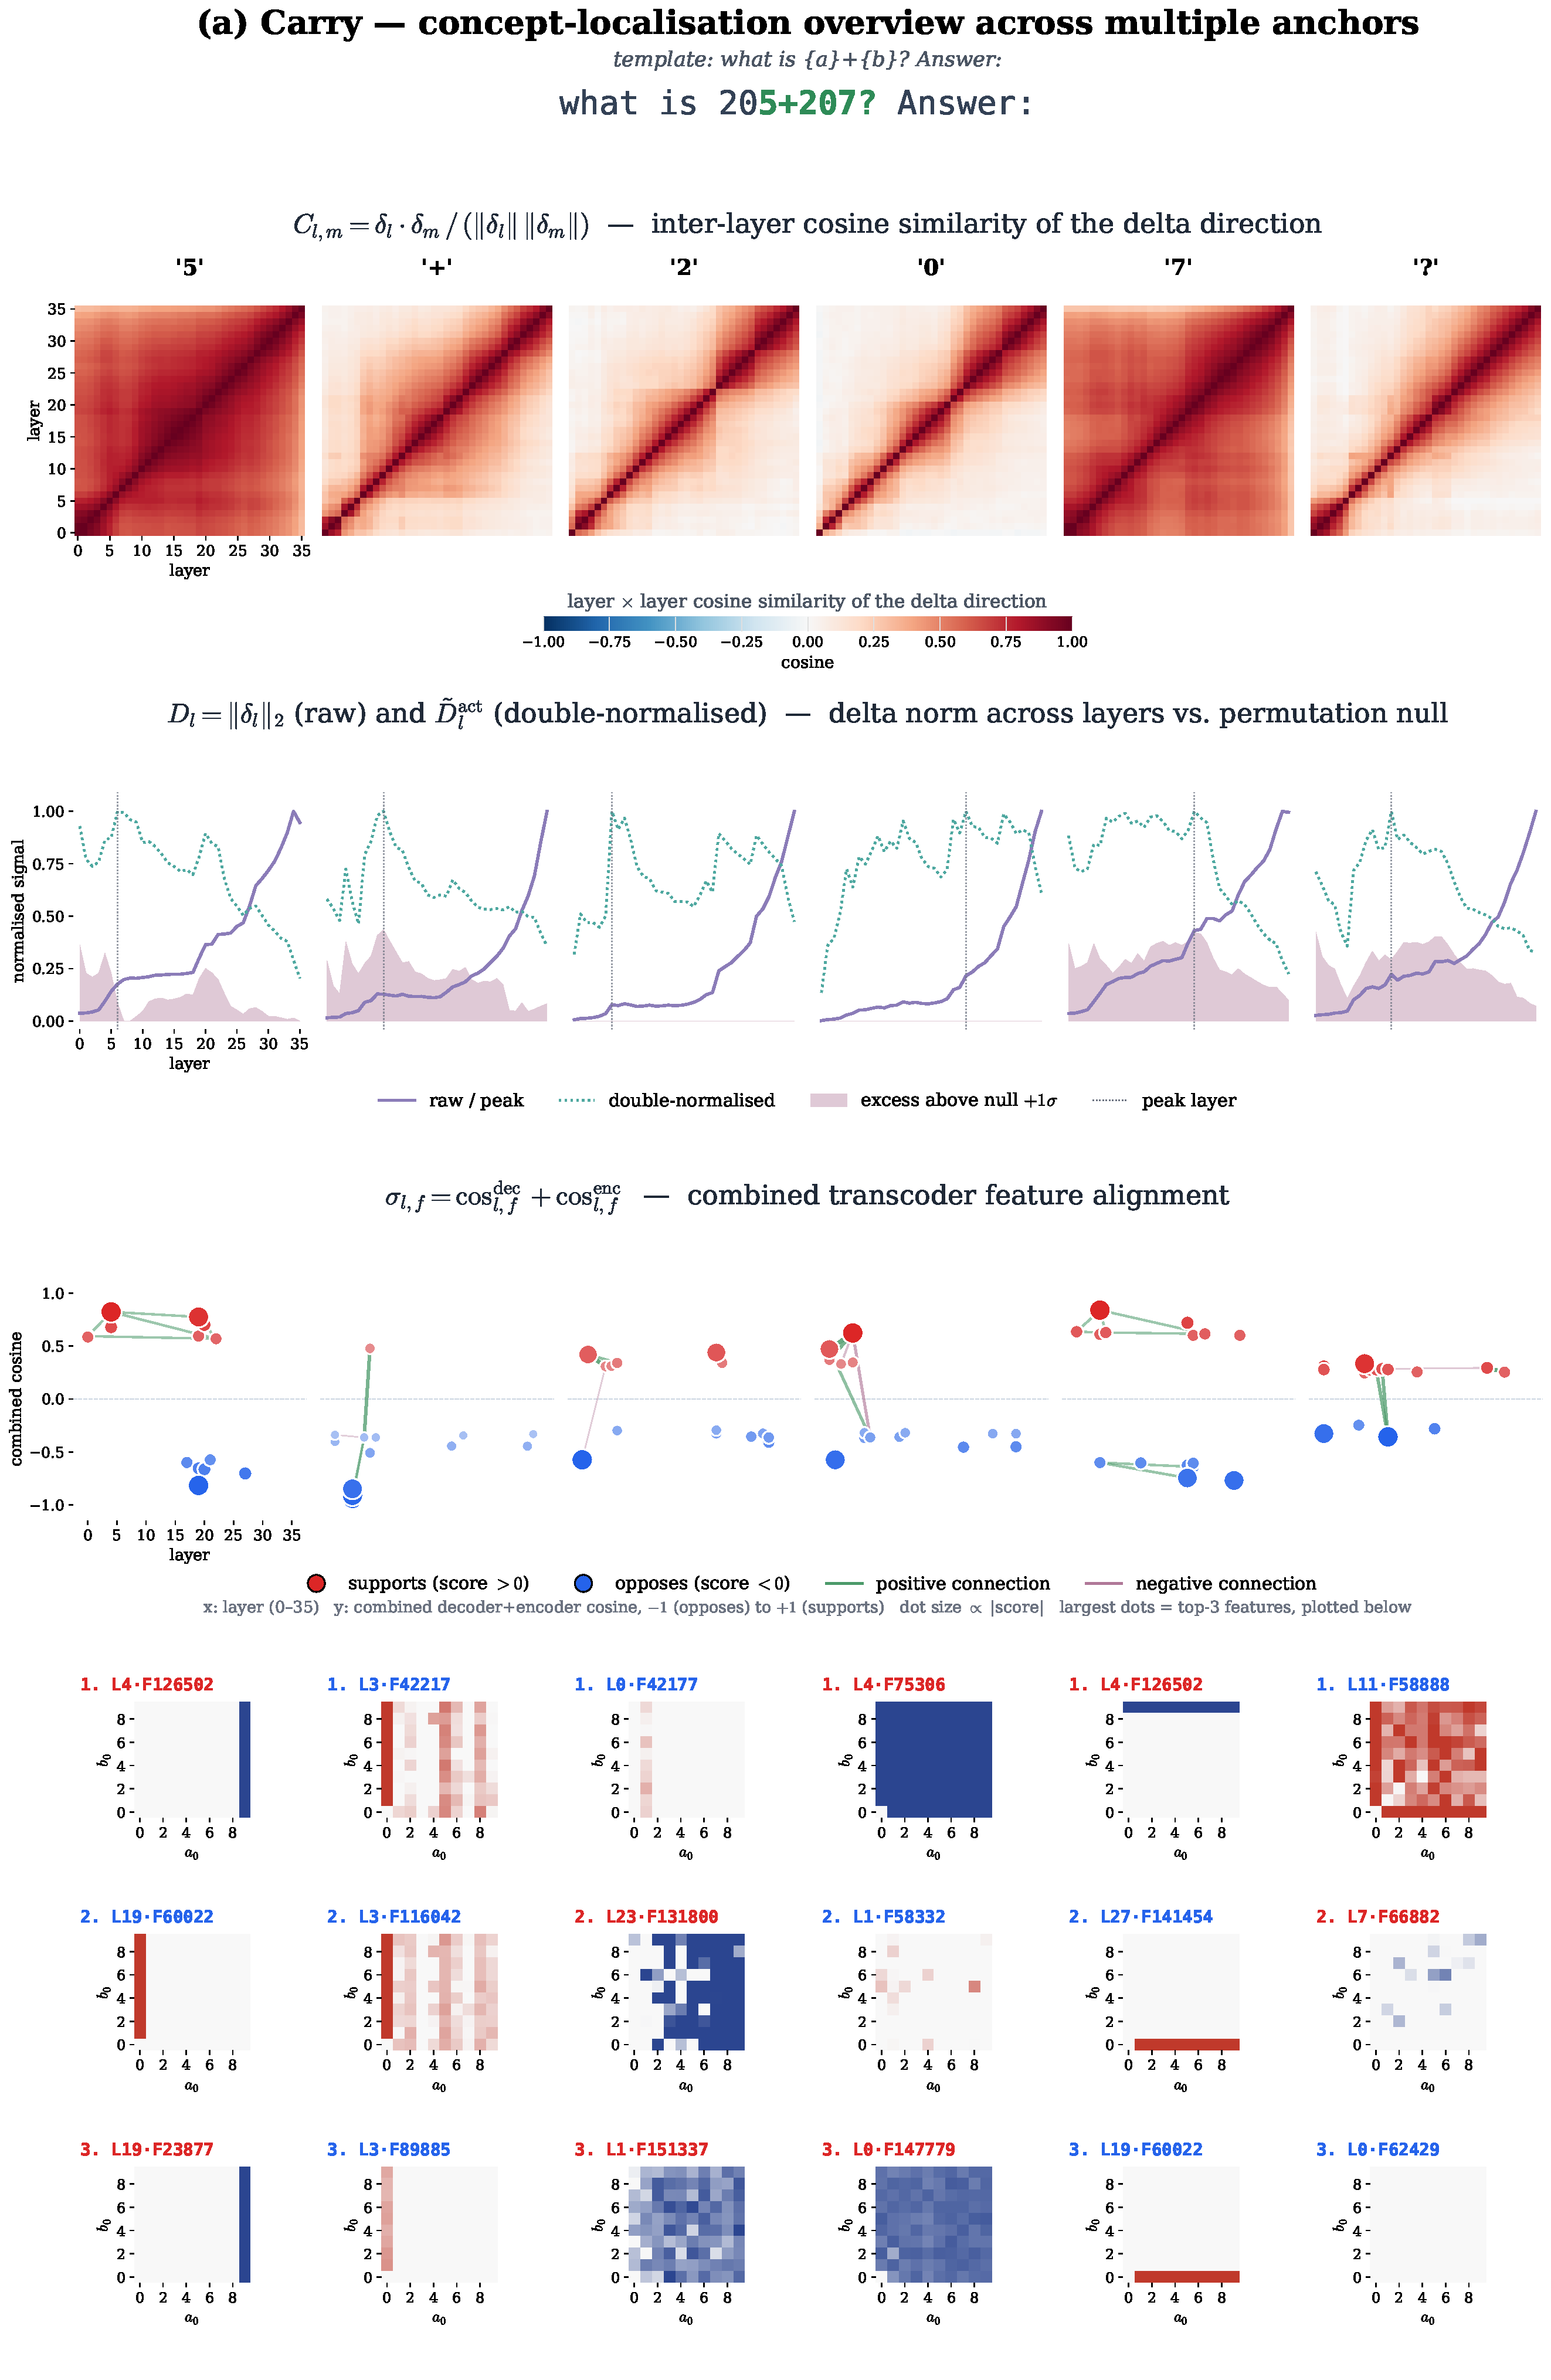
\includegraphics[width=\textwidth]{Pages/Figures/carry/concept_overview_T0_thesis.pdf}
\vspace*{\fill}
\end{figure}
\clearpage

\begin{figure}[p]
\centering
\thispagestyle{empty}
\vspace*{\fill}

\includegraphics[width=\textwidth]{Pages/Figures/gcd/concept_overview_T0_thesis.pdf}
\vspace*{\fill}
\end{figure}
\clearpage

\begin{figure}[p]
\centering
\thispagestyle{empty}
\vspace*{\fill}

\includegraphics[width=\textwidth]{Pages/Figures/residue_class/concept_overview_T0_thesis.pdf}
\vspace*{\fill}
\end{figure}
\clearpage

\begin{figure}[p]
\caption[Concept-localisation overview across all anchors, for carry, GCD, and residue class]{%
Concept-localisation overview across all six anchors for each of the three concepts
defined in Table \ref{tab:concept_pairs}, in order:

\medskip
\noindent(a) \textbf{Carry} (\promptinline{what is~\{a\}+\{b\}?~Answer:~}).
Across all distinct features shown for the six anchors, the great
majority are single-digit selectivity detectors firing for a specific
ones-digit of $a$ or $b$ (e.g.\ $a_0=9$). Sometimes, they are gated by the other digit
being non-zero or diffuse features without digit-pair structure. The
cosine-similarity panels show high-similarity blocks for
ones$_a$ and ones$_b$ anchors, consistent for all layers, and suggesting stable 
concept representation at these positions.
The other anchors in this figure show diffuse diagonals, indicating gradual 
rotation of the carry direction across layers. Since the model uses ones$_a$ and ones$_b$ 
to compute the carry (as shown using ablation in Table \ref{tab:carry_intervention}), 
it is expected that the model has a \textit{high-vs-low} digit magnitude direction at these anchors, as
high digits are more likely to produce a carry than low digits. 
\label{fig:concept_overview_carry}

\medskip
\noindent(b) \textbf{GCD divisibility} (\promptinline{the~gcd~of~\{a\}~and~7~is:~}).
Divisibility-by-seven detectors can be seen once the model
reads ones$_a$ by layer 10, where a clear block rotation also appears. Here, the model
does not yet read the operator (seven). However, the contrastive nature of our
experiment reveals divisibility-by-seven features, indicating that the model has
already learned a divisibility-by-seven representation for arbitrary integers, which
it can later use to compute the GCD once the operator is read. This resembles predictive preactivation in human language comprehension, where contextual
expectations can probabilistically activate representations of likely upcoming input before that
input is encountered \citep{kuperberg2016prediction}. Here, however, the anticipated content
appears to be computationally specific rather than a lexical identity (e.g. 
anticipation of the token \texttt{7}).

The delta trajectory row shows null-excess bands at anchors starting from ones$_a$, 
and the inter-layer cosine matrix shows a block transition at layer
 10 for the ones$_a$ anchor, 
 where projected features start exhibiting prime (e.g. $L^{10}_{74500}$, $L^{22}_{88709}$, $^{22}_{24461}$) and 
 co-prime ($L^{13}_{12887}$) patterns by seven.

 \label{fig:concept_overview_gcd}

\medskip
\noindent(c) \textbf{Residue class} (\promptinline{calc:~\{a\}\%7=~}). The
delta trajectory row shows that the concept signal does not rise 
above the permutation-null
mean$+1\sigma$ band. This suggests that the residue class concept 
is not binary, in contrast
to the other concepts studied here. Most of the
features read out below each constellation are, again, divisibility-by-seven
detectors rather than detectors of the nominally selected class
$a\equiv 1\pmod 7$.
\label{fig:concept_overview_residue}
}
\end{figure}